INTRO
%\VV{I suggest we use a 1) Introduction. 2) Methods. 3) Results 4) Discusssion -structure. }
%\VV{Many good poitns here, and thorough work on the literature! I think we should focus on writing a "mathemacial biology/modeling paper. There, the structure can be generalized as follows. Intro: 1) What is the background of our work. This is well defined in our current intro. 2) What has been done on the subject before. We have to foucs on both experiments and mathematical modeling. \\

% General presentation of the paper and its objective before writting more details 
%\VV{I think the intro covers everything we need now. Good job! My recommendation would be to shorten and sharpen the introduction a bit. If we do: 1) Intro to subject e.g. short about glymphatics 2) then some experimental studies 3) Modeling studies 4) What has not been done in modeling and open questions. 5) How does our study contribute to solve the open questions? We don't have to follow this recipe, but it can be used to shorten it down a bit. I think we can manage to have the intro stop on page 2.} 
% Make sure we follow guidelines (looks good so far).  https://journals.plos.org/plosone/s/submission-guidelines#loc-cell-lines


%Many biological experiments have been conducted to study these questions, we here cover only a few of them. The interested reader can find many references in the recent reviews~\cite{Holter9894,abbott_role_2018,jessen_glymphatic_2015}. 

%Therefore, there is a need of a macroscopic description of the glymphatic system capable to retain information from the micro-scale.
%One option could be to use a perfusion model. They often combine one dimensional structures, \ie the vessels, embedded in a three dimensional porous medium, \ie the tissue. A coupling between the two types of structures represent the exchange of fluid and solutes between the vessels and the tissue.
%Such mathematical models have been used to study .
%Even though this modelling framework allows to retain a lot of information from the micro-scale, its main drawback is that a complete description of the vessel tree is required. At the scale of the total brain, such information is often impossible to obtain and is highly restricted by the resolution of the imaging technique. Furthermore, the cerebral vasculature may not fixed in time as it evolves to adapt to specific constraints (\eg cerebral tumors~\cite{Jabin-arterial-2022}). 

%Homogenization is a mathematical method that allows to rigorously average the microscopic properties of a system to derive equations modelling its macroscopic behavior. Considering the modelling of the Glymphatic system, the different compartments must be considered: the PVS around arteries, veins, and the interstitium (more details can be found in Section~\ref{sec:method}). The homogenization process is performed from an averaging of microscopic the equations describing the micro-scale behavior occurring in the different compartments over periodic cells in the domain to end up with equations describing the behavior of the system at the macroscopic scale. 
%The resulting equations often comprise coupled systems for the different compartments. 
  

% tracer movement and drug delivery
%To summarize, the mechanisms behind metabolic solute clearance remain unclear and are currently debated.% Furthermore, studies of tracer movement within the human brain from an intrathecal injection suggest that the Glymphatic system have the potential to be an efficient pathway to deliver drugs to the brain, bypassing the Blood-Brain Barrier~\cite{ringstad_brain-wide_2018}.  





% About the mathematical modelling of the Glymphatic system
% What has been done previously and what remains do be done. 
% Hence, what is our problematic? What is the lock? 

%\paragraph{Mathematical and computational modelling}
%Biological experiments to study the Glymphatic system are often difficult to perform and very costly when not impossible. Therefore, accessing the mechanisms explaining the observed flow of CSF and movement of solutes in the brain remains a challenge.
%For these reasons, mathematical modeling of the Glymphatic system  has the potential to help unveiling the possible mechanisms behind biological observations and orient future researches. Computational fluid dynamics models have addressed the importance of arterial pulsations for fluid movement in the PVS (\eg~\cite{daversin-catty_mechanisms_2020,Diem-2017-pulsation,Ladron-2020-bc,Thomas-2019-fluid}), and convection-diffusion equations have allowed for  studies on molecular transport at the scale of the brain~\cite{ray_analysis_2019,valnes_apparent_2020,Holter9894,nicholson-1981-ion, stoverud_modeling_2012}. These latter works helped gain some insights of the relevant mechanisms that may play a role for clearance of interstitial solutes. Their main conclusion is that it is unlikely that clearance is explained solely by diffusion within the parenchyma.   

  

%Modelling the Glymphatic system accurately at the scale of the total brain while retaining the capacity to perform efficient numerical simulations asks the question of the level of details needed.
%Depending on the type of application, often a compromise has to be made between accuracy and efficiency.

%To represent vessels and tissue, perfusion models is one choice. 

%For these reasons, one efficient solution is to use homogenized models. 

%The derivation of these mathematical models often relies on the assumptions that the microscopic features of the system are distributed periodically within the medium. 
%Each of these structures, \ie the microscopic features and the medium, are considered as different compartments with specific properties. 


% MPET and ventikos
%In this work, we consider the brain tissue to be a solid matrix. This simplifying assumption is of course untrue and, hence, a more realistic modelling framework would consider deformations. To this end, Multiple-network poroelastic theory (MPET in short) has been applied. This latter theory has been developed for geomechanics applications (see \eg~\cite{Biot-1941-Consolidation,Biot-1955-Consolidation2} for single fluid network and~\cite{Bai-MPET-1993} for multiple fluid networks) and has been recently used to represent fluid movement in the brain~\cite{tully_ventikos_2011,Vardakis-2016-cerebral,Guo-2018-MPET,Guo-2019-MPET}. 
%These models are derived from a continuum approach: starting from mass balance equation of fluid density in each compartment, a set of equations is found for fluid pressures in each compartment. These latter equations are coupled to an equation modelling elastic deformation of the medium (\ie the brain tissue). The coupling between the compartments lies in appropriate transfer functions modelling the transport of fluid due to pressure differences.
%We emphasise that the previously cited works using the MPET do not consider solute transport. 

%We denominate our model the \textit{MPT model} (for \textit{Multiple-Porosity Theory}). 
%Even though the model is general enough the consider different types of mechanisms (\ie convection, diffusion, membrane conditions), it retains information at the microscopic scale and allows for different properties in each compartment. %The equations system can be obtained from homogenization of a microscopic description of the Glymphatic system and assuming a periodic distribution of vessel throughout the brain or, in a simpler manner, from a continuum approach. 
%The model derivation presented in this article follows the second method.
%To access the relevancy of such modelling framework, we compare the results obtained with the standard convection-diffusion equation (within one compartment) to our multi-compartment model for the representation of solute clearance in the rat brain. In particular, we consider the important molecule \Cinulin. 
%The latter is known to not cross the Blood-Brain Barrier (BBB in short). 
%It is assumed that this molecule is cleared from the brain by diffusion or by the Glymphatic system. 
%To study these different pathways, we consider three test cases in which different effects explain the clearance. In the first test case, clearance is obtained only by diffusion in the extra-cellular space. In the second test case, the Glymphatic system is assumed to conntribute to clearance. In the third, we also consider the contribution of blood perfusion to the fluid movement and study the resulting clearance assuming that \Cinulin can be cleared by blood.
%These three test cases are represented in Figure~\ref{fig:multi-comp}.

METHODS

%In Section~\ref{sec:method}, we present and motivate the mathematical models that we use. We introduce the initial and boundary conditions, carefully chosen to approximate the biological experiments. This section contains also the parameters' definitions and values for fluid movement and \Cinulin diffusion as well as convection.
%Section~\ref{sec:results} presents the numerical results and compares the simulation results with biological data. 
%In Section~\ref{sec:discussion}, we use this section to discuss the relevancy of the mathematical models as well as its advantages compared to other models from the literature.      

%Using variations of our model and numerical simulations, fluid flow computed from the multi-compartment model considering the Glymphatic system to be isolated from the influence of blood perfusion, revealed flow in the ECS compartment into the brain, and clearance was thus slightly delayed compared to pure diffusion. In cases where PVS were enlarged, clearance was increased, but within a reasonable physiological range of PVS radii, the increase of clearance after 6 hours was limited to 8\% of the total amount injected. Taking into account the effect of blood perfusion on the CSF movement, convection in PVSs was largely increased and we found a difference of 0.44\%  of cleared solute with the case in which the Glymphatic system as an isolated system.

\commentout{
\paragraph{The pressure equation.}
To represent the movement of the interstitial fluid, we use a compressibility relation that links the density of the fluid $\rho = \rho(t,\x)$ to its pressure $p_e = p_e(t,\x)$ (see Appendix~\ref{app:derivation} for the details of this computation). The time-space evolution of the pressure is given by
\begin{equation}
    C_e \frac{\partial p_e}{\partial t} +  \nabla\cdot( v_e ) +  C_e v_e  \cdot \nabla p_e = 0,\quad \forall x\in \Omega,\quad t\in (0,T],
    \label{eq:pressure-1comp}
\end{equation}
in which $C_e$ is the compressibility coefficient.  
}


%This work is the first step toward bridging the gap between microscopic properties of the Glymphatic system and an efficient macroscopic modelling of fluid and solute transport within the brain. 

%\paragraph{Darcy's law. } To define the velocity field in Equation~\eqref{eq:diffusion-convection}, we use Darcy's law~\cite{darcy1856fontaines} of movement that stipulates that the velocity field is proportional to the the opposite of the gradient of the fluid's pressure, \ie  
%\begin{equation}
%\vel_e = -\f{\kappa_e}{\mu_e} \nabla p_e,
%\end{equation}
%where $\kappa_e$ is the permeability coefficient for the fluid in the interstitial space and $\mu_e$ is the dynamic viscosity of the fluid. 


%\VV{1) Diffusion convection equation. 2) Multiple compartment diffusion convection. 3) Velocities in 2) will come from MPT (list equations). }

%We now describe the modeling of clearance of \Cinulin using Equation~\eqref{eq:diffusion-convection} and/or System~\eqref{eq:main-system}. 
%This molecule is of interest because it is known to not cross the BBB and its clearance could use different routes. Indeed, it is unclear if \Cinulin is cleared only from diffusion in the ECS or if the Glymphatic system plays a role.


%Since \Cinulin is not able to cross the blood-brain-barrier, molecules injected into the brain parenchyma will be confined to the ECS compartment.
%It is not clear if \Cinulin injected into the frontal cortex of rats is confined in the interstitial space and is cleared from this compartment. Differences in clearance rates between the sleeping and awake state have been observed in mice~\cite{Xie_2013_sleep}. 

%The difference of applied pressure between the different PVS compartments is explained by our aim to produce a bulk flow that represents the Glymphatic system , \ie inflow around arteries and outflow around veins.


%The boundary conditions for the compartments $j \in \{e,pa,pc,pv\}$ is then given by Equation~\eqref{eq:inulin-boundary-inhomogeneous}.
%\begin{remark}
%We do no consider time dependent Dirichlet boundary conditions for the multi-compartment model since, as shown by our numerical results in Section~\ref{sec:results}, the type of boundary conditions does not play a big role for the time scale considered in our study. 
%\end{remark}
%The interstitial space and perivascular spaces are in communication with the subarachnoid space. Therefore, as in the previous description of the boundary conditions for\Cinulin, we need to compute the concentration within the CSF in the subarachnoid space.


%From the previous parameter values and assuming the same surface density for the PVSs as for the blood vessels, we have
%\[
%\begin{aligned}
%    &L_{pa,e} = \gamma_{e, pa} \frac{\abs{\Omega}}{\abs{S_{pa,e}}} = 3.5 \times 10^{-8}  \text{mm/(s.Pa)},\quad  L_{pc,e} = \gamma_{e, pc} \frac{\abs{\Omega}}{\abs{S_{pc,e}}} = 5.3 \times 10^{-11}  \text{mm/(s.Pa)},\\
%    &L_{pv,e} = \gamma_{e, pv} \frac{\abs{\Omega}}{\abs{S_{pv,e}}} = 3.2 \times 10^{-8}  \text{mm/(s.Pa)}.
%\end{aligned}
%\]

%\AP{Maybe reduce sigma that to model change of width between big vessels and smaller ones.}
%\AP{TODO: Find references for this statement. }


%\paragraph{\Cinulin}
%Using a free diffusion coefficient for \Cinulin of $ D = 2.98 \times 10^{-6} \text{cm}^2/ \text{s} $ as reported in \cite{lanman1971diffusion}, and a tortuosity of $ \lambda=1.7 $ \cite{Waters-2011-AB}, the effective diffusivity of \Cinulin in the ECS is given by
%\[ 
%  D_{ \text{eff}} = \frac{D}{\lambda^2} = 1.03\times 10^{-6} \text{cm}^2/ \text{s}.
%\]

\commentout{
\paragraph{The effect of blood vessels}
In the usual picture of the Glymphatic system, the leakage or resorption of fluid from the blood vessels is not considered. However, even though the BBB is known to be a tight selective barrier, a small amount of fluid can cross the membrane of blood vessels. The hydraulic conductivity of capillaries, arterioles and venules have been measured in different species and is known to not be zero (see \eg~\cite{fraser1990measurement, kimura1993measurement, roberts2009ppar}). We consider the effect of fluid leakage from the blood vessel in the third test case corresponding to an application of the model~\eqref{eq:main-system} with 7 compartments. The baseline parameter values for the fluid flow are given in Table~\ref{tab:fluid} and for the transfer between compartments in Table~\ref{tab:exchange}. We highlight here that no transfer of \Cinulin from PVS to the blood is considered since this molecule is known to not cross the BBB.
}

RESULTS
\commentout{
\VV{Searching through literature, it seems they report mouse CSF production in nl/min. I found 100 nL/min in~\cite{liu2020direct}.}In other words, it means that every hour, the periarterial space transfers $0.03 \si{mL}$ of CSF to the extracellular space (\ie roughly $13.3\%$ of CSF circulates in the ECS in 1 hour\VV{reference for this?}). 
}

\commentout{
 \begin{figure}[htbp]
     \centering
     \begin{subfigure}[t]{0.45\textwidth}
         \captionsetup{width=0.9\textwidth}
         \centering
         %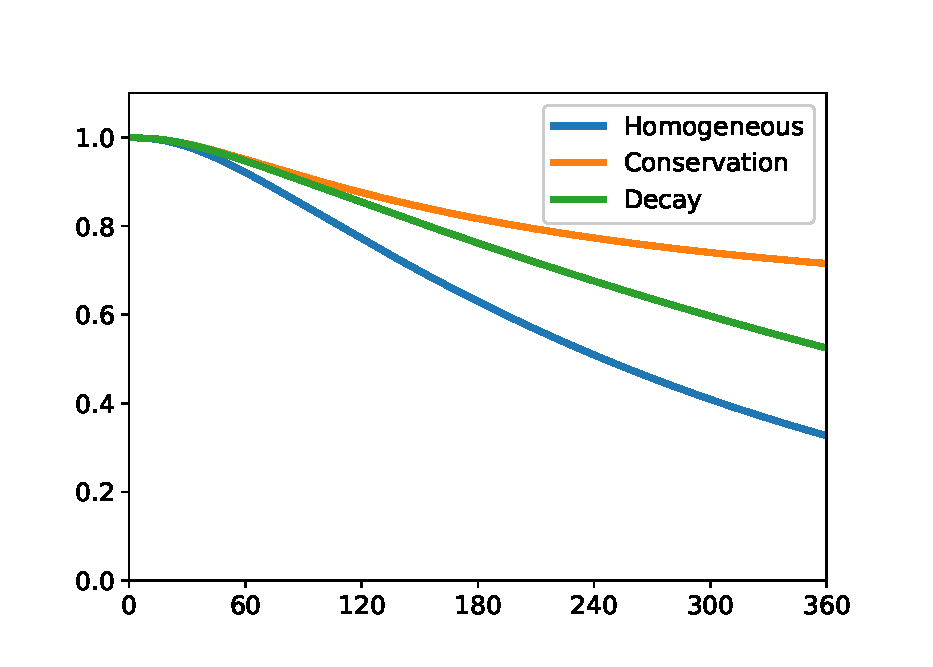
\includegraphics[width=\textwidth]{images/boundaries/bound-diff-final.eps}
         \caption{Single diffusion equation}
         \label{fig:diffusion-bcs-Inulin}
     \end{subfigure}
     \hfill
     \begin{subfigure}[t]{0.45\textwidth}
         \captionsetup{width=0.9\textwidth}
         \centering
         %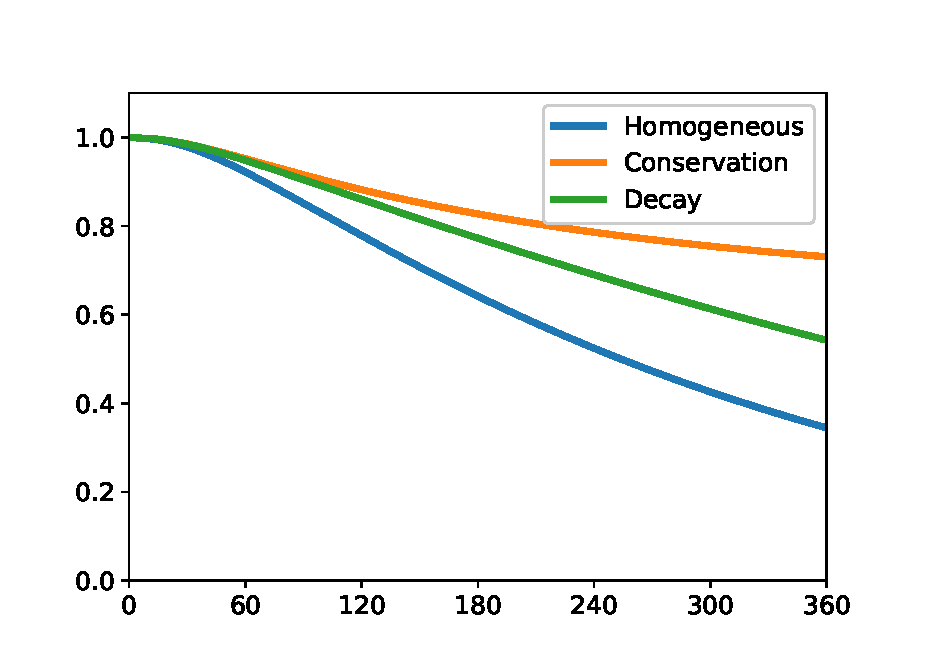
\includegraphics[width=\textwidth]{images/boundaries/bound-multicomp-final.eps}
         \caption{Multi-compartment model.}
         \label{fig:multi-compartment-bcs-Inulin}
     \end{subfigure}
     \caption{Relative \Cinulin mass located in the totality of the brain for the different boundary conditions.}
     \label{fig:bcs-Inulin}
\end{figure}



\commentout{
\begin{figure}[htbp]
\centering
     \begin{subfigure}[b]{0.49\textwidth}
         \centering
         %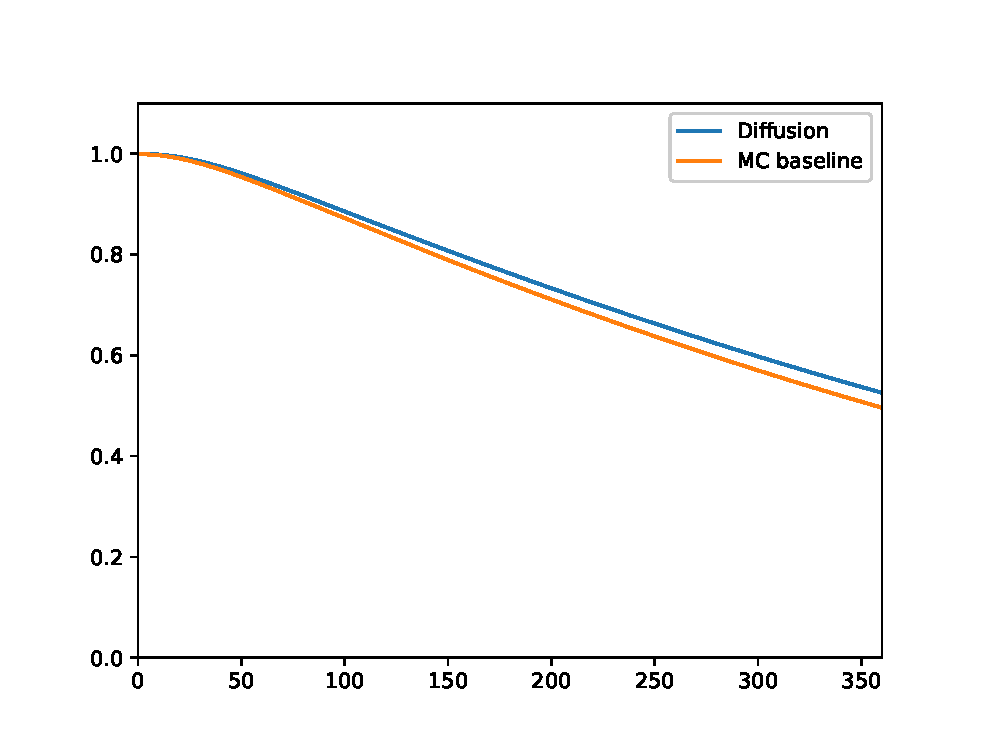
\includegraphics[width=0.95\textwidth]{images/Inulin-multcomp/compare-baselines.eps}
         \caption{Evolution in time of the relative mass of \Cinulin in the brain for \Cinulin test cases 1 (Diffusion) and 2 (MC baseline).}
         \label{fig:compare-clear-inulin-baselin}
     \end{subfigure}
     \hfill
      \begin{subfigure}[b]{0.49\textwidth}
         \centering  
         %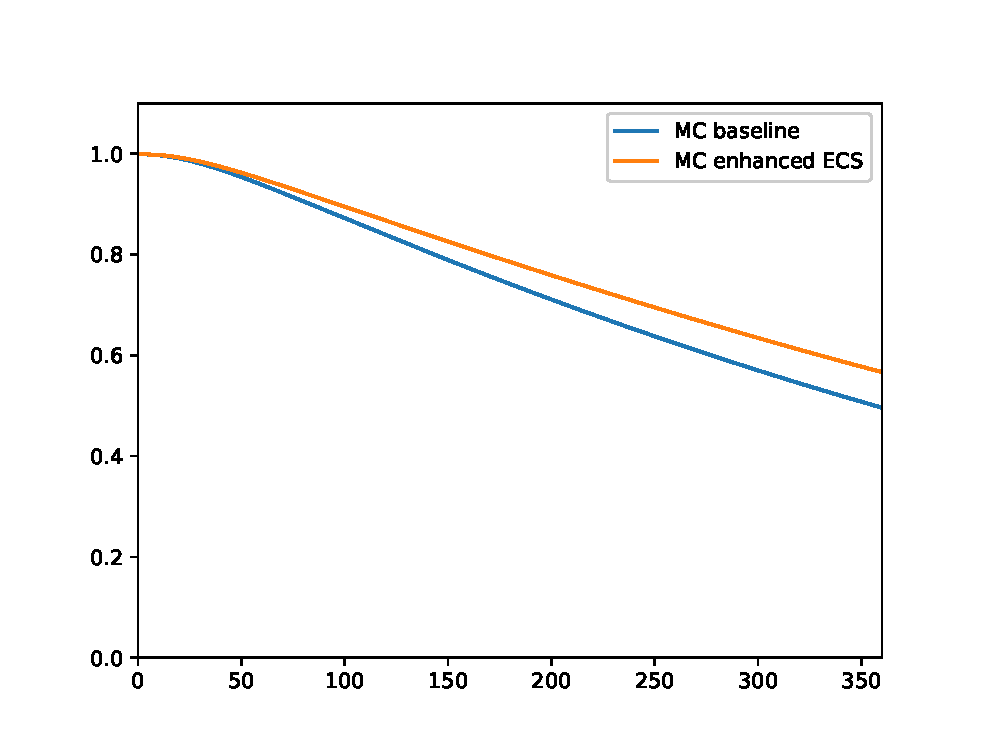
\includegraphics[width=0.95\textwidth]{images/Inulin-multcomp/compare-inulinECS.eps}
         \caption{Evolution in time of the relative mass of \Cinulin in the brain for \Cinulin test cases 2 with baseline parameters (MC baseline), enhanced porosity and permeability in  ECS (MC enhanced ECS).}
         \label{fig:compare-clear-inulin-enhancedECS}
        \end{subfigure}
        
        \begin{subfigure}[b]{0.49\textwidth}
         \centering  
         %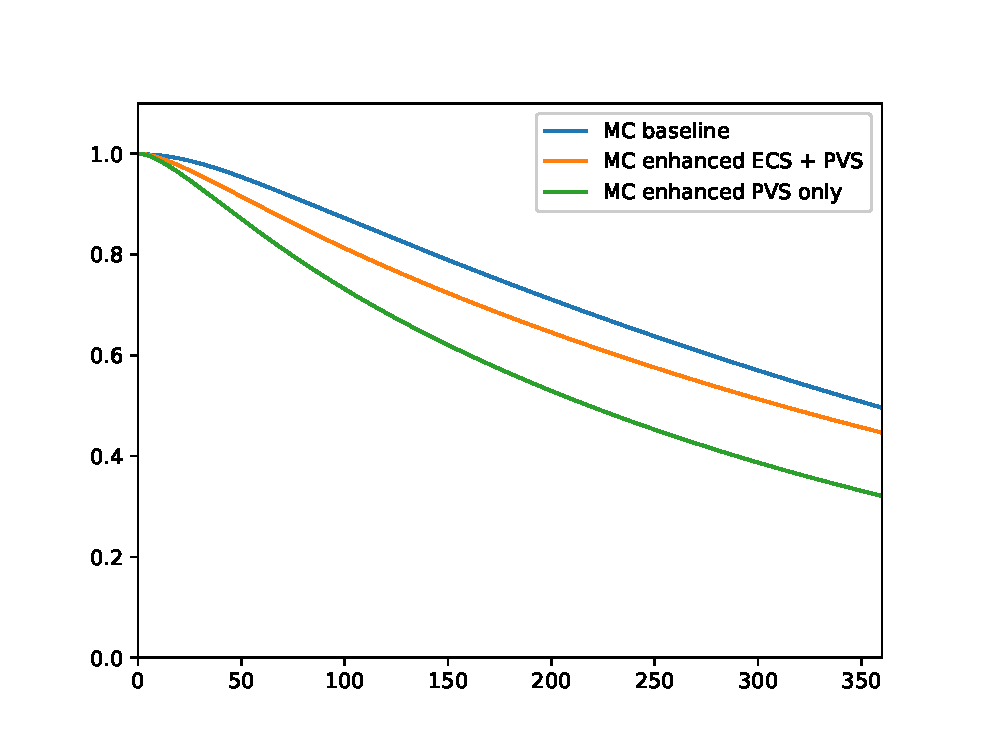
\includegraphics[width=0.95\textwidth]{images/Inulin-multcomp/compare-inulinPVS.eps}
         \caption{Evolution in time of the relative mass of \Cinulin in the brain for \Cinulin test cases 2 with baseline parameters (MC baseline), combined enhanced porosity and permeability in PVSs and ECS (MC enhanced ECS + PVS), and enhancement in the PVSs only (MC enhanced PVS only).}
         \label{fig:compare-clear-inulin-enhancedPVS}
        \end{subfigure}
        
        \caption{Comparison of \Cinulin clearance for different variations of porosity and permeability coefficients. \VV{I think we can have one figure with all curves in it. Also put on legends}}
\end{figure}
}


\commentout{
 \begin{figure}[htbp]
     \centering
     \begin{subfigure}[t]{0.45\textwidth}
         \captionsetup{width=0.9\textwidth}
         \centering
         %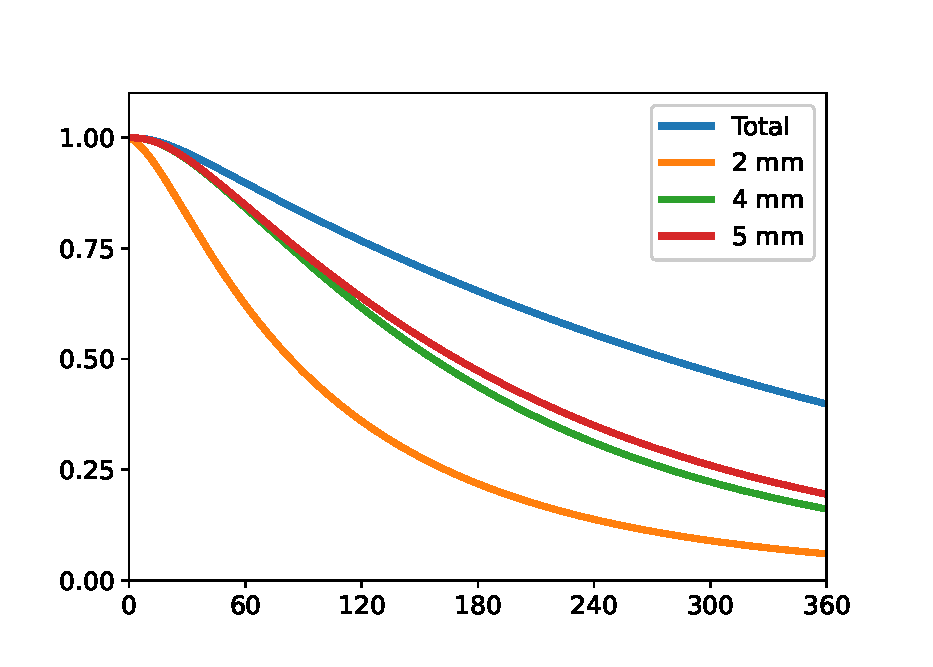
\includegraphics[width=\textwidth]{images/samples/samples-final-diffusion.eps}
         \caption{Single diffusion equation}
         \label{fig:diffusion-samples-Inulin}
     \end{subfigure}
     \hfill
     \begin{subfigure}[t]{0.45\textwidth}
         \captionsetup{width=0.9\textwidth}
         \centering
         %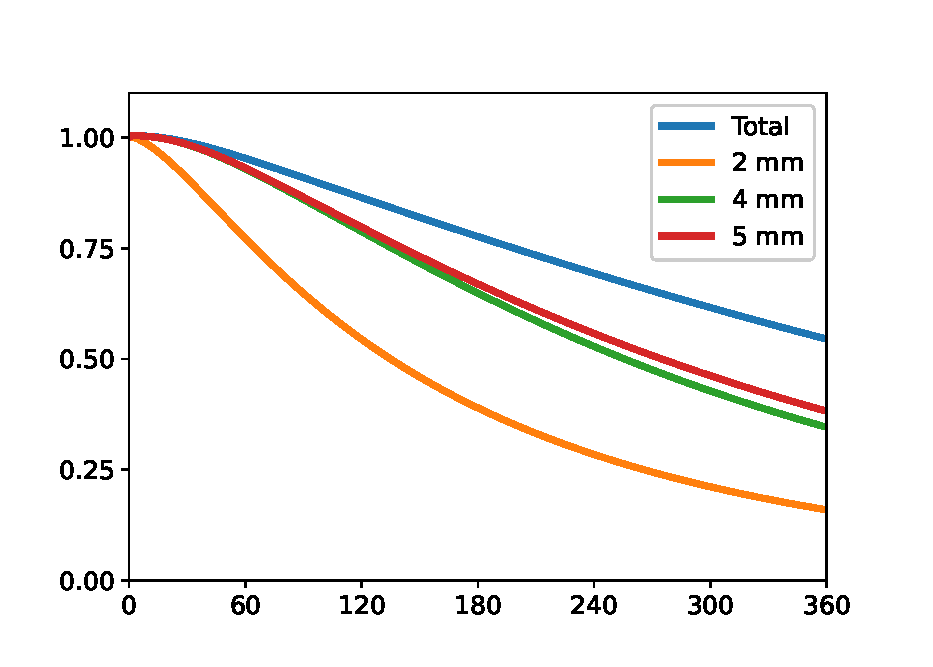
\includegraphics[width=\textwidth]{images/samples/samples-final-4multicomp.eps}
         \caption{Multi-compartment model.}
         \label{fig:multi-compartment-samples-Inulin}
     \end{subfigure}
     \caption{Relative \Cinulin mass located within regions of varying size surrounding the injection point. \VV{Figures need axis labels}}
     \label{fig:samples-Inulin}
\end{figure}
}

% Fig~\ref{fig:compare-poro} compares the clearance of \Cinulin given by the multi-compartment model with baseline coefficients, the multi-compartment model combining the enhanced porosities and permeabilities coefficients in the ECS (see the previous subsection) as well as PVSs.

\commentout{
\begin{figure}[htbp]
         \centering
         %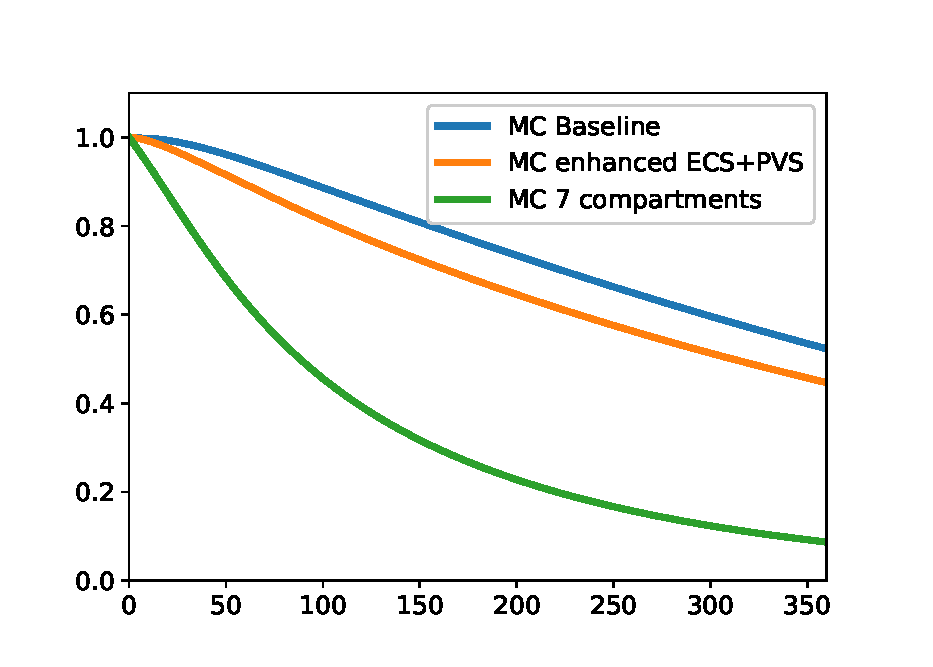
\includegraphics[width=0.6\textwidth]{images/final-clearance-blood.eps}   
        \caption{Comparison of \Cinulin clearance for test case 2 with baseline parameter values and increase of ECS and PVSs porosities with test case 3. "MC Baseline" denotes the clearance curve given by the multi-compartment model with baseline parameter values. The enhancements of ECS and PVSs porosities lead to the curve denoted "MC enhancement ECS+PVS", and the result of test case 3 is denoted "MC 7 compartments"}
        \label{fig:compare-blood}
\end{figure}
}
\begin{figure}[htb]
    \centering
    %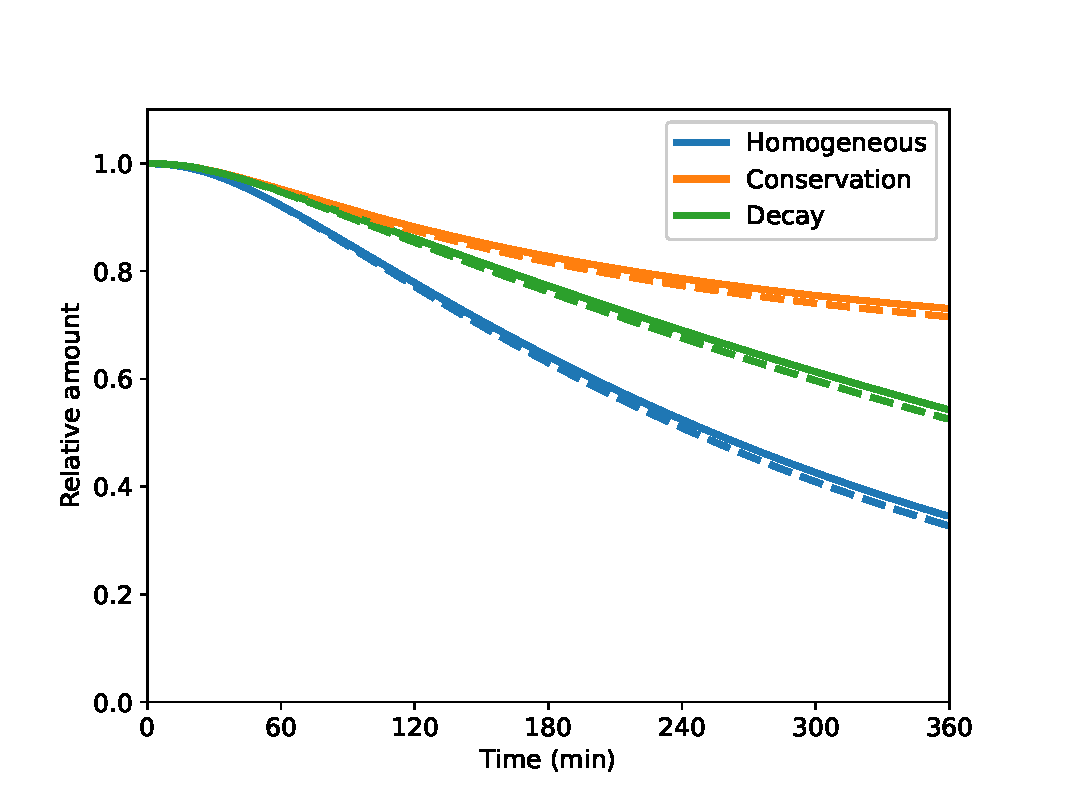
\includegraphics[width=0.6\textwidth]{images/final-boundaries.eps}
    \caption{Relative \Cinulin mass located in the totality of the brain for the different boundary conditions. Solid lines result from the multi-compartment model simulations, while dashed lines result from diffusion only in the ECS.}
   \label{fig:bcs-Inulin}
\end{figure}
}

% maybe use later
%Fig~\ref{fig:compare-poro} compares the clearance curves of \Cinulin for Test cases 1 and 2 with baseline parameter values. We observe that no significant differences can be found between the two models for the baseline parameter values. However, varying the porosities in the different compartments leads to changes in the clearance of the \Cinulin.

